\documentclass[dvipsnames, 9pt]{beamer}

%\documentclass[xcolor=dvipsnames, 8pt]{beamer} %
%\setbeamertemplate{navigation symbols}{}

\usetheme{SantaBarbara}

%light gray/black highlighting to be used with pause command
\colorlet{shadecolor}{gray!40}
\def\blackgray<#1>{%
  \temporal<#1>{\color{shadecolor}}{\color{black}}{\color{shadecolor}}}

\definecolor{black}{HTML}{0A0A0A}
\definecolor{red}{HTML}{e00404} 


\definecolor{blue}{HTML}{0647A8}
\definecolor{darkgreen}{HTML}{008000}

\definecolor{Asparagus}{HTML}{87A96B}

\usepackage[utf8]{inputenc}
\usepackage{algorithm, algpseudocode}

\usepackage{tightlist}
\usepackage{tikz, tikzsettings}
\usepackage{verbatim}
\usepackage{amssymb}
\usepackage{amsmath}
\usepackage{amsfonts}
\pdfmapfile{+sansmathaccent.map} % Fix done for making the talk in ubuntu.
\graphicspath{{./}{./figures/}{./figures/presentation/}}
\usepackage{makecell}
\usepackage{booktabs}

\usepackage{subcaption}
\usepackage[authoryear,round]{natbib}
\usepackage{color}
\usepackage{colortbl}
\usepackage{xcolor}
\usepackage{pgfplots}
\usepackage{ragged2e}
\usepackage{rxn}
\usepackage{hyperref}


\usetikzlibrary{shapes,calc,spy, calc, backgrounds,arrows, fit, decorations.pathmorphing, decorations.pathreplacing, matrix}
\usepackage{caption}
\usepackage{mpcsymbols}
\usepackage{graphicx}

\newcommand{\calert}[1]{\textcolor{blue}{#1}}

\makeatother
\setbeamertemplate{footline}
{\leavevmode%
	\hbox{%
		\begin{beamercolorbox}[wd=.3\paperwidth,ht=2.25ex,dp=1ex,center]{author
		in head/foot}%
			\usebeamerfont{author in head/foot}\insertshortauthor
		\end{beamercolorbox}%
		\begin{beamercolorbox}[wd=.6\paperwidth,ht=2.25ex,dp=1ex,center]{title
		in head/foot}%
			\usebeamerfont{title in head/foot}\insertshorttitle
		\end{beamercolorbox}%
		\begin{beamercolorbox}[wd=.1\paperwidth,ht=2.25ex,dp=1ex,center]{date in
		head/foot}%
			\insertframenumber{} / \inserttotalframenumber\hspace*{1ex}
	\end{beamercolorbox}}%
	\vskip0pt%
}

\renewcommand{\vec}{\textnormal{vec}} 
\newcommand{\stoi}{\text{\boldmath $\nu$}}


\title[NODEs]{Stirring Up Neural ODEs: A Chemical Engineer's perspective}


\author[ME255NN--Dake]{Prithvi Dake}
\institute [UCSB]{Department of Chemical
Engineering\\
\pgfuseimage{ucsb-logo}}

\date{ME255NN Report  \\
\today}

%\AtBeginSection[]
%{
%  \begin{frame}
%    \frametitle{Outline}
%    \tableofcontents[currentsection]
%  \end{frame}}


\begin{document}

\frame{\titlepage}

\begin{frame}{Gentle intro with a simple problem}
    \begin{columns}
    {\begin{column}{0.45\textwidth}
    \begin{block}{}
        Consider following \textcolor{red}{\textit{true}} model of linear chemical kinetics taking place
        in a well-mixed batch reactor with $c = (c_A, c_B, c_C)^T$ and initial concentration
        $c_0$:
        \begin{rxn*}{} 
        A \rlh[k_1][k_{-1}] 2 B, \qquad  B \rarrow[k_2] C
        \label{rxn:atobtoc}
        \end{rxn*}
        \begin{gather*}
        \begin{bmatrix} \dot{c}_A \\ \dot{c}_B \\ \dot{c}_C \end{bmatrix}
        =\begin{bmatrix}
            -k_{1} & k_{-1} & 0 \\
            2k_{1} & 2k_{-1} - k_2 & 0 \\
            0 & k_{2} & 0
        \end{bmatrix}
        \begin{bmatrix}  c_A \\ c_B \\ c_C \end{bmatrix} 
        \label{eq:atobtoc}
        \end{gather*}
    \end{block}
    \end{column}}
    {\begin{column}{0.5\textwidth}
    \begin{figure}[h]
        \centering
        \includegraphics[width=\textwidth, page=7]{ABC_plot.pdf} 
    \end{figure}
    \end{column}}
    \end{columns}
\end{frame}

\begin{frame}{Background: If PINNs why NODEs? }
    \textbf{Training a Physics-Informed Neural Network (PINN) \footnote{\cite{raissi:perdikaris:karniadakis:2019}}}
    \begin{algorithmic}[1]
        \State \textbf{Input:} Neural network architecture $f_{NN}$
        \State \textbf{Physical Model:} $Lx=f \quad B_1 x = 0 \quad B_2 x = 0$
        \Comment{True or known physics}
        \State \textbf{Initialize} neural network parameters $\theta$
        \Repeat
            \State $x = f_{NN}(x,t; \theta)$
            \State $V_{ODE} = \norm{Lx - f}^{2}$ 
            \Comment{Prediction error minimization} 
            \State $V_{BC} = \norm{B_1 x}^{2} + \norm{B_2 x}^{2}$
            \Comment{Enforce boundary conditions}
            \State $V = \lambda_1 V_{PDE}  + \lambda_2 V_{BC}$
            \Comment{Combine loss terms}
            \State $\theta \leftarrow \theta - \eta \nabla_{\theta} V$
            \Comment{Update $\theta$ using gradient descent}
        \Until{convergence criteria is met}
        \State \textbf{Return} trained model $f_{NN}$
    \end{algorithmic}
\end{frame}

\begin{frame}{Background: If PINNs why NODEs?}
    \begin{columns}
    {\begin{column}{0.5\textwidth}
    \begin{figure}[h]
        \centering
        \includegraphics[width=\textwidth, page=8]{ABC_plot.pdf} 
    \end{figure}
    \end{column}}
    {\begin{column}{0.45\textwidth}
    \begin{block}{}
        \begin{itemize}  % Right triangle symbol
            \item I view PINNs as a softer version\footnote[frame]{By softer I 
            mean PINNs minimize rather than exactly satisfy equality constraints } of \textit{method of weighted residuals}.
            \footnote[frame]{\cite{villadsen:stewart:1967}}
            \item Mostly used as surrogate numerical solver for PDEs.
            \item Can learn some physics but has no \textit{structure}.
            \item Causality problem (no sequential model, future depends on past).
            \footnote[frame]{\cite{wang:shyam:paris:2022}}
        \end{itemize}
    \end{block}
    \begin{block}{Recent advances}
        Physics-informed neural ODE (PINODE) \footnote[frame]{\cite{sholokhov:liu:mansour:nabi:2023}} \\
        Lift-and-embed: Koopman operators \footnote[frame]{\cite{liu:sholokov:mansour:nabi:2024}}
    \end{block}
    \end{column}}
    \end{columns}
\end{frame}

\begin{frame}{ResNets and RNNs}
    \begin{block}{A state-space representation: Euler discretized system}
    \begin{align*}
        x^+ &= x + f_{NN} (x, u; \theta) &\qquad x^+ = f_{NN} (x, u; \theta)\notag \\ 
        y &= g_{NN} (x, u; \theta) &\qquad y = g_{NN} (x, u; \theta)
        \label{eq:resrnn}
    \end{align*}
    Parallels with FIR and ARX models in system identification \footnote[frame]{\cite{ljung:1999}}.\\
    Backprop strategy: Brute-force chain rule (store intermediate states).
    \end{block}
    \begin{columns}
    {\begin{column}{0.6\textwidth}
    \begin{figure}
        \centering
        \includegraphics[width=0.8\textwidth, page=2]{ABC_plot.pdf}
    \end{figure}
\end{column}}
{\begin{column}{0.3\textwidth}
    \ If $x\in\R^n, \theta\in \R^p$, $S = \dfrac{\partial x}{\partial \theta^T}\in\R^{n\times \textcolor{red}{p}}$
\end{column}}
\end{columns}
\end{frame}

\begin{frame}{Don't want to store intermediate states? Forward sensitivities for IVPs \footnote{Derivation in \cite{rawlings:ekerdt:2020}}}
    \begin{itemize}
    \item Consider a non-linear state-space model ($y=x$):
    \begin{align*}
        \dot{x} &= f(x, u; \theta) \qquad x(0) = g(x_0; \theta)
    \end{align*}
    \item Sensitivity is defined as and evolves as \footnote{Using Clairaut's Theorem on Mixed Partials}:
    \begin{align*}
        S &= \dfrac{\partial x}{\partial \theta^T} \\
        \dfrac{d S}{dt} &= \dfrac{d}{dt} \left(\dfrac{\partial x}{\partial \theta^T}\right) =
        \dfrac{\partial}{\partial\theta^T} \left(\dfrac{d x}{dt}\right) = 
        \dfrac{\partial }{\partial \theta^T} f
    \end{align*}
    \item Augmented system of ODEs:
    \begin{align*}
        \begin{bmatrix} \dot{x} \\ \dot{S} \end{bmatrix} = 
        \begin{bmatrix} f \\ \dfrac{\partial f}{\partial x^T}S + \dfrac{\partial f}{\partial \theta^T} \end{bmatrix}
        \qquad
        \begin{bmatrix} x(0) \\ S(0) \end{bmatrix} =
        \begin{bmatrix} x_0 \\ \dfrac{\partial g}{\partial \theta^T} \end{bmatrix}
    \end{align*}
    \item Notice again: $S\in \R^{n\times p}$ i.e sensitivities we need to solve
    for increase \textcolor{red}{linearly} with $p$. Imagine how bad this could get for FNN with millions of parameters and 
    states!
    \end{itemize}
\end{frame}


\begin{frame}{How to avoid the linear cost? Pontryagin's adjoint method}
    \begin{figure}
        \centering
        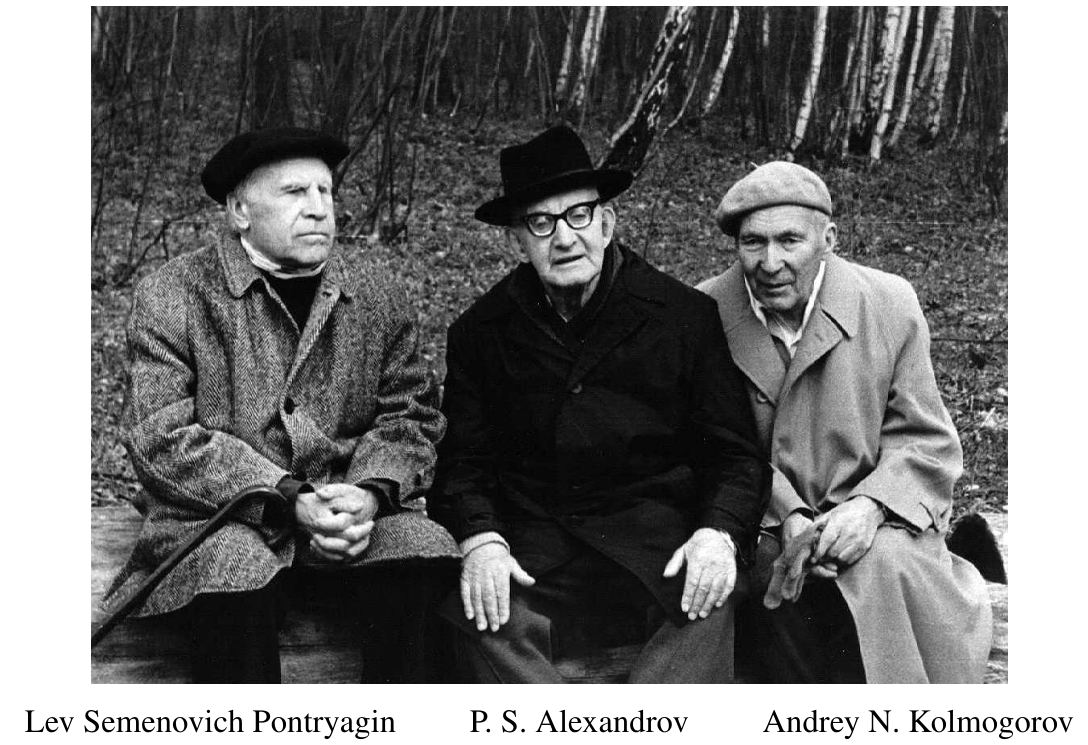
\includegraphics[width=0.8\textwidth]{oldies.png}\\
        %\textit{One mastered control, one shaped space, one gambled with certainty}.\\
    \end{figure}
\end{frame}

\begin{frame}{Backward adjoint method}
    \begin{itemize}
        \item Consider following optimization problem and the Lagrange functional given data $\tilde{x}$:
        \begin{align*}
            \min\limits_{\theta}V(x) &= \int_0^t \norm{x - \tilde{x}}^2 dt = \int_0^t g(x)dt \notag \\
            \min\limits_{\theta, \lambda}\mathcal{L} &= \int_0^t g dt + \int_0^t \lambda(t)^T \left(f - \dfrac{dx}{dt}\right) dt
        \end{align*}
        \item The augmented system of ODEs is \footnote{Refer \cite{sengupta:friston:penny:2014} for paper and 
        \url{https://youtu.be/k6s2G5MZv-I?si=ZIyP7MvgzTK7D9kn} for a walkthrough. Additionally, 
        I have worked out the derivation step-by-step in my report.}:
        \[
        \begin{bmatrix} \dot{x} \\ \dot{\lambda^T} \end{bmatrix} = 
        \begin{bmatrix} f_{NN} \\ -\lambda^T \dfrac{\partial f_{NN}}{\partial x^T}\end{bmatrix}
        \qquad
        \begin{bmatrix} x(t) \\ \lambda^T(t) \end{bmatrix} =
        \begin{bmatrix} x_t \\ - \dfrac{\partial g}{\partial x^T}|_{t} \end{bmatrix}
        \label{eq:augsens}
        \]
        \item The gradient of loss wrt parameters is calculated as:
        \[
            \dfrac{\partial V}{\partial \theta^T} = \lambda^T(0)\dfrac{\partial x}{\partial \theta^T}|_0 + \int_0^t   \lambda^T \dfrac{\partial f}{\partial \theta^T} dt
        \]
    \end{itemize}
\end{frame}

\begin{frame}{An ultimate panacea?}
    \begin{columns}
    {\begin{column}{0.45\textwidth}
    \begin{figure}
        \centering
        \includegraphics[width=\textwidth, page=4]{ABC_plot.pdf}
    \end{figure}
    \end{column}}
    {\begin{column}{0.5\textwidth}
    \begin{block}{}
        \begin{itemize}
            \item Consider $\dot{\lambda} = \pm 10 \lambda$ and $\lambda(0) = 0$
            \item We see that the adjoint variable will either \textit{explode} or 
            \textit{vanish}.
            This heavily impacts the learning problem. 
            \item The Jacobian $\dfrac{\partial f}{\partial x^T}$ can be ill-conditioned.
            \item We solve the adjoint equation by quadrature, thus numerical noise 
            can still be a problem.
        \end{itemize}
    \end{block}
    \begin{block}{Remedies}
        \begin{itemize}
            \item Don't solve adjoint over long horizons, but rather 
            small windows and store the initial conditions for those intermediate
            windows.
            \item Popularly called as \textit{checkpointing} \footnote[frame]{\cite{zhuang:dvornek:li:tatikonda:papademetris:duncan:2020}}.
        \end{itemize}
    \end{block}
    \end{column}}
    \end{columns}
\end{frame}

\begin{frame}{NODE}
    \begin{algorithmic}[1]
        \State \textbf{Input:} Neural network architecture $f_{NN}$
        \State \textbf{ODE:} 
        $
            \begin{bmatrix} \dot{x} \\ \dot{\lambda^T} \end{bmatrix} = 
            \begin{bmatrix} f_{NN} \\ -\lambda^T \dfrac{\partial f_{NN}}{\partial x^T}\end{bmatrix}
            \qquad
            \begin{bmatrix} x(t) \\ \lambda^T(t) \end{bmatrix} =
            \begin{bmatrix} x_t \\ - \dfrac{\partial g}{\partial x^T}|_{t} \end{bmatrix}
            \label{eq:augsens}
        $
        \Comment{Construct the augmented ODE using \texttt{PyTorch}}
        \State \textbf{Initialize} neural network parameters $\theta$
        \Repeat
            \State $V = \norm{\hat{x} - x}^2$
            \Comment{Forward solve to get the loss $V$}
            \State $\hat{x}_{aug} = \text{ODESolve}(f_{aug}, x_{aug}(0), T, t_0)$
            \State $\dfrac{\partial V}{\partial \theta^T} = \lambda^T(0)\dfrac{\partial x}{\partial \theta^T}|_0 + \int_0^t   \lambda^T \dfrac{\partial f}{\partial \theta^T} dt$
            \Comment{Construct the gradient wrt loss}
            \State $\theta \leftarrow \theta - \eta \nabla_{\theta} V$
        \Until{convergence criteria is met}
        \State \textbf{Return} trained model $f_{NN}$
        \end{algorithmic}        
\end{frame}

\begin{frame}{NODE}
    \begin{figure}
        \centering
        \includegraphics[width=0.65\textwidth, page=1]{ABC_plot.pdf}\\
        Concentration profiles of species A, B, and C in a batch reactor. The
    NODE model also does quite a good job to predict the concentration profiles. 
    In fact for such simple problem, we hardly see any difference between ResNet and NODE
    \footnote{All the case studies in this report are built using \texttt{Torchdiffeq} by \cite{torchdiffeq}}.
    \end{figure}
\end{frame}

\begin{frame}{Generative latent model using CNF}
    \begin{itemize}
        \item \textbf{Latent} = States in state-space model, since we usually cannot measure
        them directly. Thus, we construct state-estimators.
        \item \textbf{Generative latent} = State-space model that also propagates uncertainty
        in estimates i.e. you can sample and \textit{generate} multiple trajectories after learning.
        \item Surprise! Good old Kalman filter can be called a generative latent model!
        \footnote{Refer \cite{rawlings:mayne:diehl:2020} for derivation of the Kalman filter using
        Bayesian estimation principles.}
        \item Consider a simple linear transform:
        \begin{align*}
            x &\in \mathcal{N}(m, \sigma^2 I) \\
            y &= Ax \\
            y &\in \mathcal{N}(Am, A\sigma^2 A^T)
        \end{align*}
        \item Bayesian approach: $\textcolor{blue}{p(y|x)} \sim p(x|y) \textcolor{red}{p(y)}$.
        Assuming an \textcolor{red}{uniform prior} the likelihood problem is 
        \[
        \theta = \arg\max\limits_{\theta} \log p(x|y; \theta) \qquad p(x|y) = A^{-1} y \sim \mathcal{N}(m, \sigma^2I)        \]
        \item Ofcourse, $A$ is assumed to be non-singular (i.e. unique mapping between $x$ and $y$;
        \textit{bijective mapping}).
    \end{itemize}
\end{frame}

\begin{frame}{Extending the bayesian framework for any non-linear transform}
    \begin{itemize}
        \item Consider following series of transformations (\textit{planar-flow}):
        \[
        x^+ = f_{NN}(x, u; \theta) \qquad x(0) \sim \mathcal{N}(m, \sigma^2I) \qquad x(t) \sim ?
        \]
        \item Use \textit{change of variables}, compute the
        \textcolor{red}{determinant} of Jacobian ($\sim N(o^3)$) and conserve the probability mass as well
        as maximize the likelihood.
        \item Instead use continuous framework (\textit{continuous normalizing flow}) \footnote{Refer \cite{chen:rubanova:bettencourt:duvenaud:2018} for proof}:
        \begin{align*}
        \dfrac{dx}{dt} = f_{NN}(x, u; \theta) &\qquad x(0) \sim \mathcal{N}(m, \sigma^2I) \qquad x(t) \sim ?\\
        \dfrac{\partial p(x)}{\partial t} &=  -\mathrm{tr}\nabla_x f_{NN}
        \end{align*}
        \item Cost to get the trace of Jacobian is now linear $\sim N(o)$
    \end{itemize}
\end{frame}

\begin{frame}{Generative latent model for kinetics}
    \begin{figure}
        \centering
        \includegraphics[width=\textwidth, page=3]{ABC_plot.pdf}\\
    \end{figure}
    \begin{align*}
        \begin{bmatrix} \dot{c}_A \\ \dot{c}_B \\ \dot{c}_C \\ \dot{\log p} \end{bmatrix}
        = \begin{bmatrix}
            -k_{1}c_A + k_{-1}c_B  \\
            2k_{1}c_A +  2k_{-1}c_B - k_2c_B \\
            k_{2}c_B\\
            -\mathrm{tr} \left(\dfrac{\partial f_{NN}}{\partial c^T}\right)
        \end{bmatrix};
        &\qquad
        \begin{bmatrix} c_A(0) \\ c_B(0) \\ c_C(0) \\ \log p(0) \end{bmatrix} =
        \begin{bmatrix} 1 \\ 0 \\ 0 \\ \log{\mathcal{N}([c_A, c_B, c_C]^T, \sigma^2I)} \end{bmatrix} \notag \\
        \min\limits_{\theta} V(c) &= -\log p(c) + \norm{c - \tilde{c}}^2
    \end{align*}
\end{frame}

\begin{frame}{Robustness analysis of NODEs \footnote{Refer \cite{yan:du:tan:feng:2019}}}
    \begin{figure}[h]
        \centering
        \includegraphics[width=0.5\textwidth, page=5]{ABC_plot.pdf} \\
        Robustness analysis of ODEs. We see that the solution $c_{B2}$ 
        is sandwiched between two perturbed solutions $c_{B1}, c_{B3}$, 
        though all approach the same steady-state. Also note that the slightly time-shifted
        solution appears as a perturbed solution \footnote{Refer \cite{ascher:petzold:1998}
        for well-posedness theorem of IVPs.}
        \label{fig:robust}
    \end{figure}
    \center \textbf{Theoretical bound}
    \begin{align*}
        \norm{x(t+T)-x(t)} \leq \norm{\int_t^{t+T} f_{NN}(x, u; \theta) dt}
    \end{align*} 
\end{frame}

\begin{frame}{How to train your NODE?}
    
\begin{figure}[h]
    \centering
    \includegraphics[width=0.55\textwidth, page=6]{ABC_plot.pdf}  \\
    If we train based only on prediction loss, the model can overfit.
    However, if we penalize the Jacobian term ($\dfrac{\partial f_{NN}}{\partial x^T}$), we can regularize the model
    to damp the oscillations \footnote{\cite{finlay:jacobsen:nurbekyan:oberman:2020} \\ 
    Access the code for all figures at \url{https://github.com/dakeprithvi/2025a_cnf}}
    \end{figure}
\end{frame}

\begin{frame}[allowframebreaks]{References}
	\renewcommand{\refname}{}
	\bibliographystyle{abbrvnat}
	%\bibliographystyle{abbrvnat_no_url}
	\bibliography{abbreviations,articles,books,proceedings, cnf_bib}
\end{frame}

\end{document}